\documentclass[../slides.tex]{subfiles}
\begin{document}

\begin{frame}{Datenerfassung: Photogammetry}
  
\begin{minipage}[t]{.5\textwidth}
    \begin{block}{Photogammetry}
        \begin{itemize}
            \item Additive Fertigung
            \item Datenerfassung
            \item Datenaufarbeitung
            \item Stitching 
            \item Deformationserkennung
            \item Algorithmus und Software
            \item Ausblick
        \end{itemize}
    \end{block}
    \end{minipage}
    \hfill
    \begin{minipage}[t]{.49\textwidth}
    \begin{figure}[]
        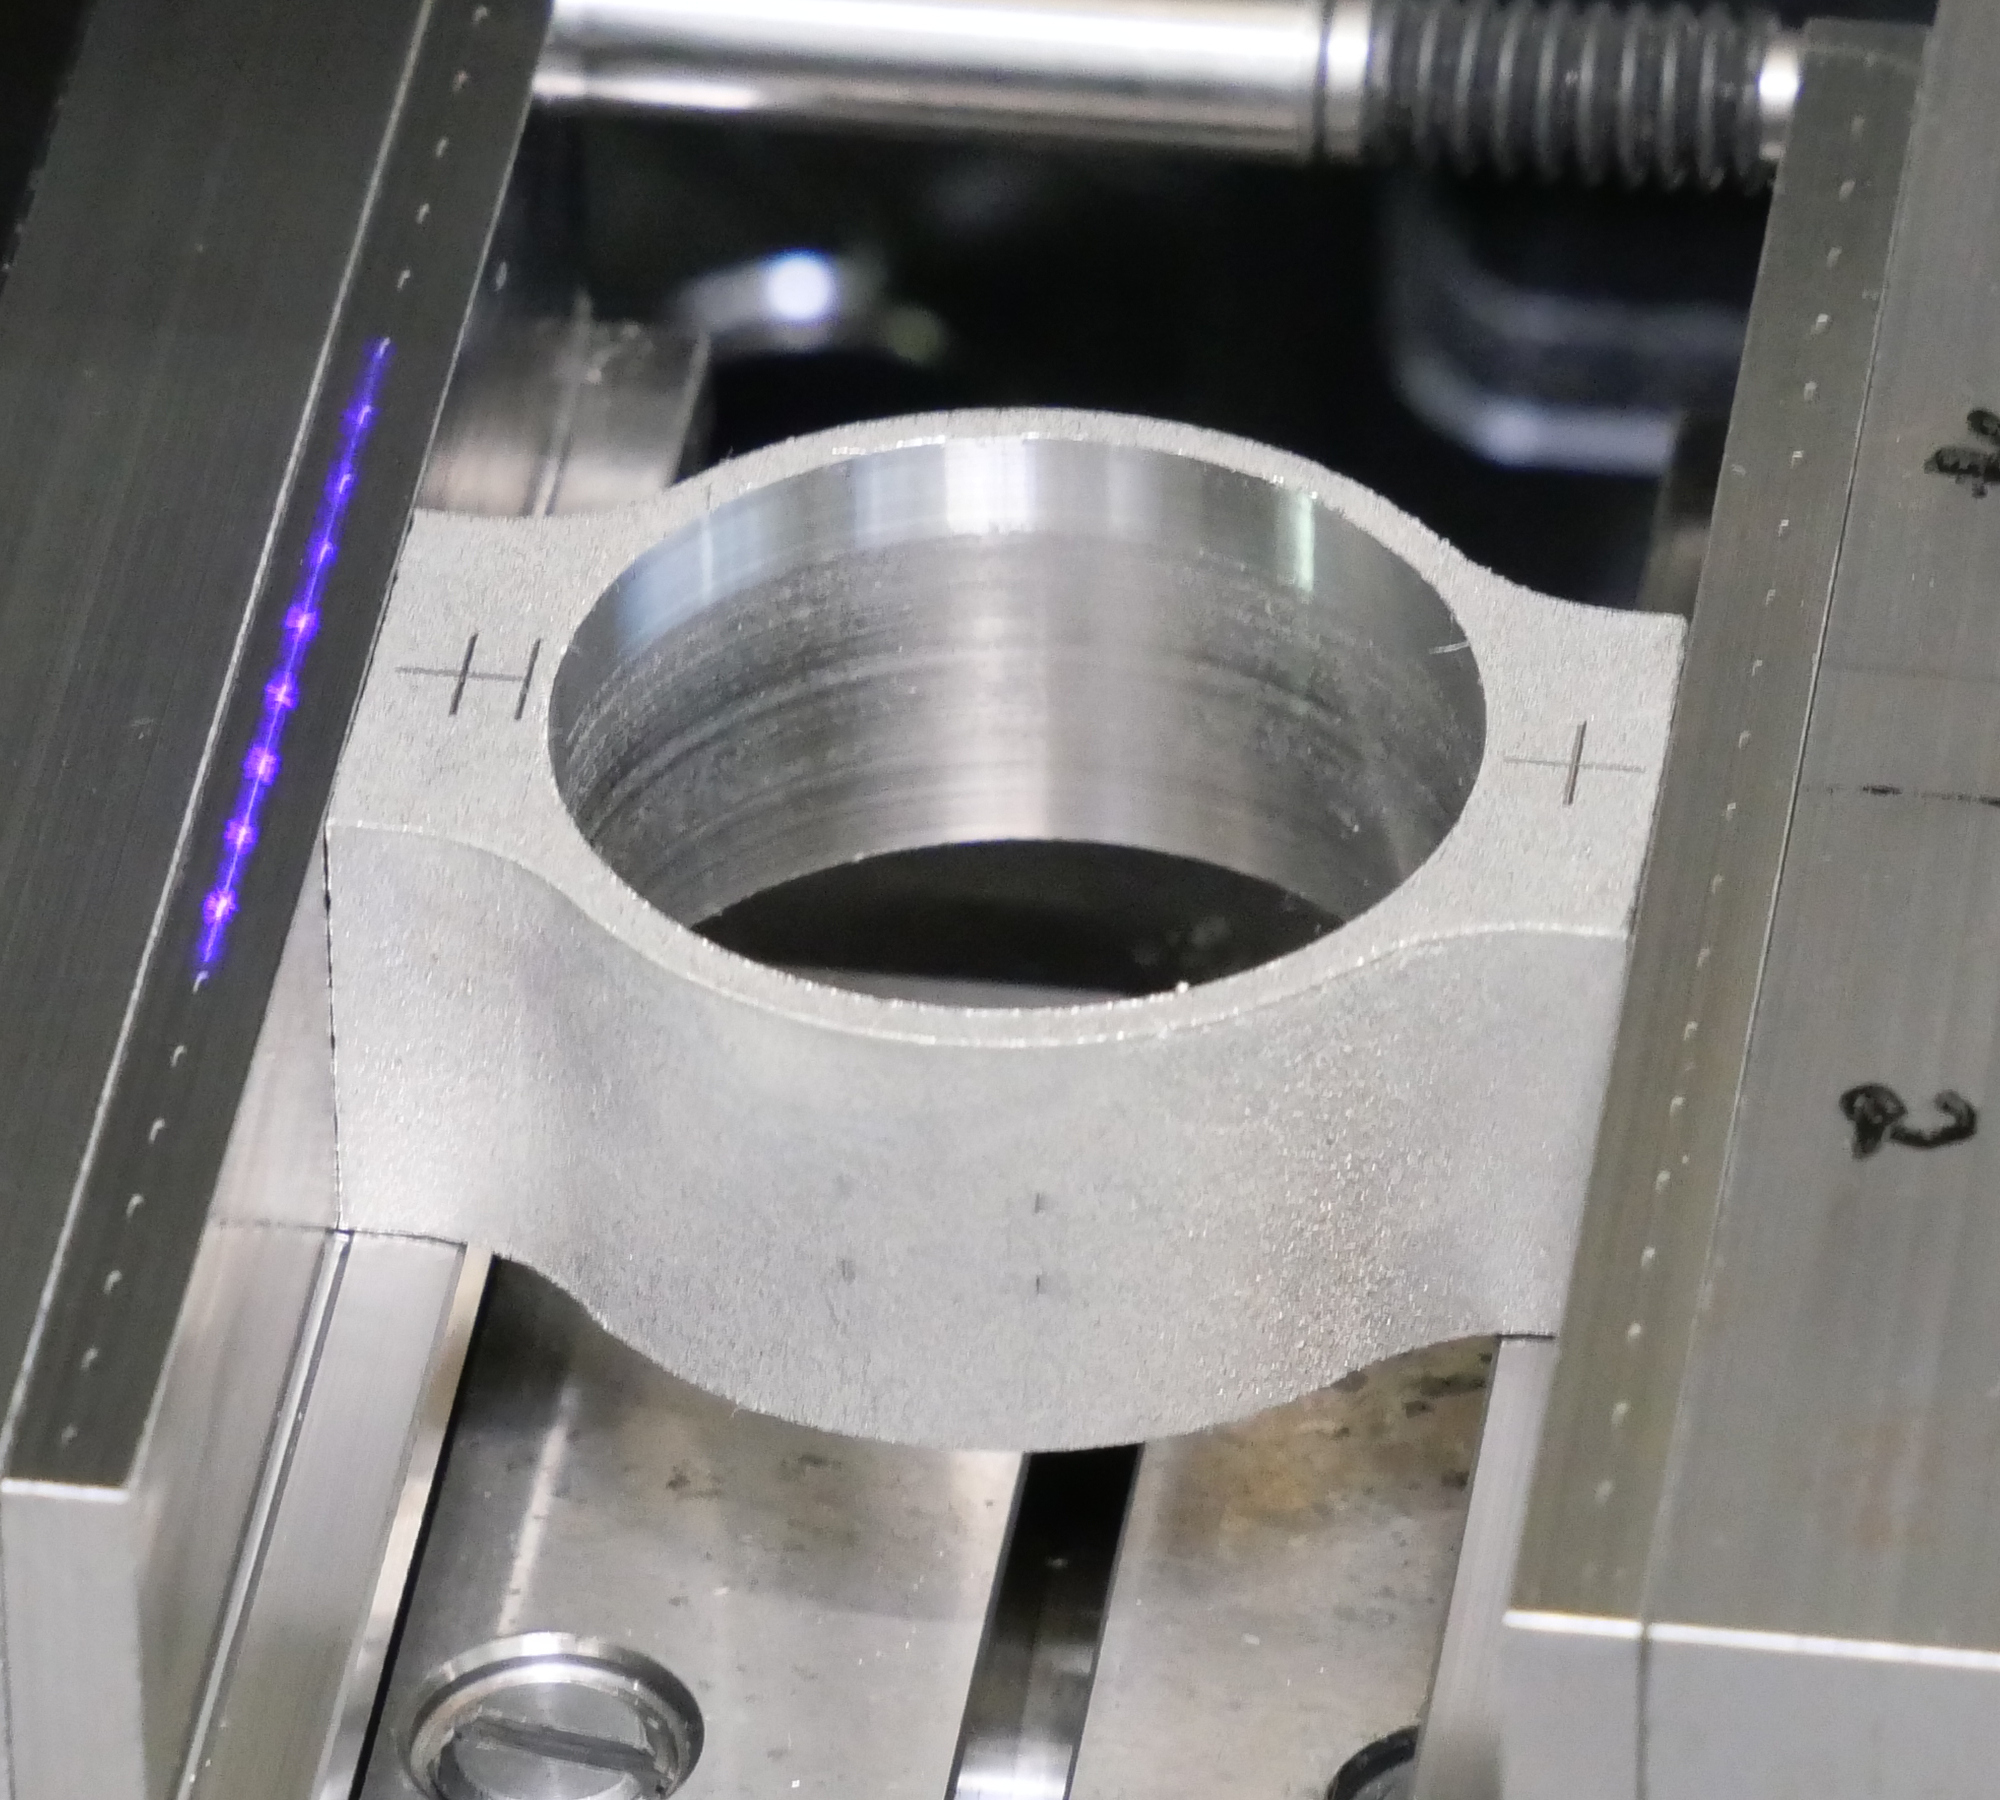
\includegraphics[height=150pt]{img_niklas/AM2_crop.JPG}
        \caption{Additiv gefertiges Demonstratorbauteil}
    \end{figure}
    \end{minipage}    
\end{frame}

\end{document}